%% Creator: Inkscape 1.2.1 (9c6d41e, 2022-07-14), www.inkscape.org
%% PDF/EPS/PS + LaTeX output extension by Johan Engelen, 2010
%% Accompanies image file 'bloch_sphere.pdf' (pdf, eps, ps)
%%
%% To include the image in your LaTeX document, write
%%   \input{<filename>.pdf_tex}
%%  instead of
%%   \includegraphics{<filename>.pdf}
%% To scale the image, write
%%   \def\svgwidth{<desired width>}
%%   \input{<filename>.pdf_tex}
%%  instead of
%%   \includegraphics[width=<desired width>]{<filename>.pdf}
%%
%% Images with a different path to the parent latex file can
%% be accessed with the `import' package (which may need to be
%% installed) using
%%   \usepackage{import}
%% in the preamble, and then including the image with
%%   \import{<path to file>}{<filename>.pdf_tex}
%% Alternatively, one can specify
%%   \graphicspath{{<path to file>/}}
%% 
%% For more information, please see info/svg-inkscape on CTAN:
%%   http://tug.ctan.org/tex-archive/info/svg-inkscape
%%
\begingroup%
\makeatletter%
\providecommand\color[2][]{%
  \errmessage{(Inkscape) Color is used for the text in Inkscape, but the package 'color.sty' is not loaded}%
  \renewcommand\color[2][]{}%
}%
\providecommand\transparent[1]{%
  \errmessage{(Inkscape) Transparency is used (non-zero) for the text in Inkscape, but the package 'transparent.sty' is not loaded}%
  \renewcommand\transparent[1]{}%
}%
\providecommand\rotatebox[2]{#2}%
\newcommand*\fsize{\dimexpr\f@size pt\relax}%
\newcommand*\lineheight[1]{\fontsize{\fsize}{#1\fsize}\selectfont}%
\ifx\svgwidth\undefined%
  \setlength{\unitlength}{177.93310547bp}%
  \ifx\svgscale\undefined%
    \relax%
  \else%
    \setlength{\unitlength}{\unitlength * \real{\svgscale}}%
  \fi%
\else%
  \setlength{\unitlength}{\svgwidth}%
\fi%
\global\let\svgwidth\undefined%
\global\let\svgscale\undefined%
\makeatother%
\begin{picture}(1,1.06027363)%
  \lineheight{1}%
  \setlength\tabcolsep{0pt}%
  \put(0,0){\includegraphics[width=\unitlength,page=1]{bloch_sphere.pdf}}%
  \put(0.2887321,0.28921972){\color[rgb]{0,0,0}\makebox(0,0)[lt]{\lineheight{0}\smash{\begin{tabular}[t]{l}$x$\\ \end{tabular}}}}%
  \put(0.97157299,0.44096214){\color[rgb]{0,0,0}\makebox(0,0)[lt]{\lineheight{0}\smash{\begin{tabular}[t]{l}$y$\end{tabular}}}}%
  \put(0.45522726,0.9935414){\color[rgb]{0,0,0}\makebox(0,0)[lt]{\lineheight{0}\smash{\begin{tabular}[t]{l}$z$\end{tabular}}}}%
  %\put(0.44047452,0.41690636){\color[rgb]{0,0,0}\makebox(0,0)[lt]{\lineheight{0}\smash{\begin{tabular}[t]{l}φ\end{tabular}}}}%
  \put(0.44047452,0.41690636){\color[rgb]{0,0,0}\makebox(0,0)[lt]{\lineheight{0}\smash{\begin{tabular}[t]{l}$\phi$\end{tabular}}}}%
  % \put(0.45101219,0.69597371){\color[rgb]{0,0,0}\makebox(0,0)[lt]{\lineheight{0}\smash{\begin{tabular}[t]{l}θ\end{tabular}}}}%
  \put(0.45101219,0.69597371){\color[rgb]{0,0,0}\makebox(0,0)[lt]{\lineheight{0}\smash{\begin{tabular}[t]{l}$\theta$\end{tabular}}}}%
  \put(0,0){\includegraphics[width=\unitlength,page=2]{bloch_sphere.pdf}}%
  \put(0.04935377,0.94994952){\color[rgb]{0,0,0}\makebox(0,0)[lt]{\lineheight{0}\smash{\begin{tabular}[t]{l} \end{tabular}}}}%
  % \put(0,0){\includegraphics[width=\unitlength,page=3]{figs/bloch/bloch_sphere.pdf}}%
  \put(0.46622932,0.0080449){\color[rgb]{0,0,0}\makebox(0,0)[lt]{\lineheight{0}\smash{\begin{tabular}[t]{l}$\ket{1}$\end{tabular}}}}%
  % \put(0,0){\includegraphics[width=\unitlength,page=4]{figs/bloch/bloch_sphere.pdf}}%
  \put(0.35242254,0.95312728){\color[rgb]{0,0,0}\makebox(0,0)[lt]{\lineheight{0}\smash{\begin{tabular}[t]{l}$\ket{0}$\end{tabular}}}}%
  % \put(0,0){\includegraphics[width=\unitlength,page=5]{figs/bloch/bloch_sphere.pdf}}%
  % \put(0.6104334,0.7732887){\color[rgb]{0,0,0}\makebox(0,0)[lt]{\lineheight{0}\smash{\begin{tabular}[t]{l}ψ\end{tabular}}}}%
  \put(0.6104334,0.7732887){\color[rgb]{0,0,0}\makebox(0,0)[lt]{\lineheight{0}\smash{\begin{tabular}[t]{l}$\ket{\psi}$\end{tabular}}}}%
\end{picture}%
\endgroup%
